\documentclass[tikz,border=8pt]{standalone}
\usepackage{amsmath,amssymb}
\usetikzlibrary{arrows.meta,calc}

\begin{document}
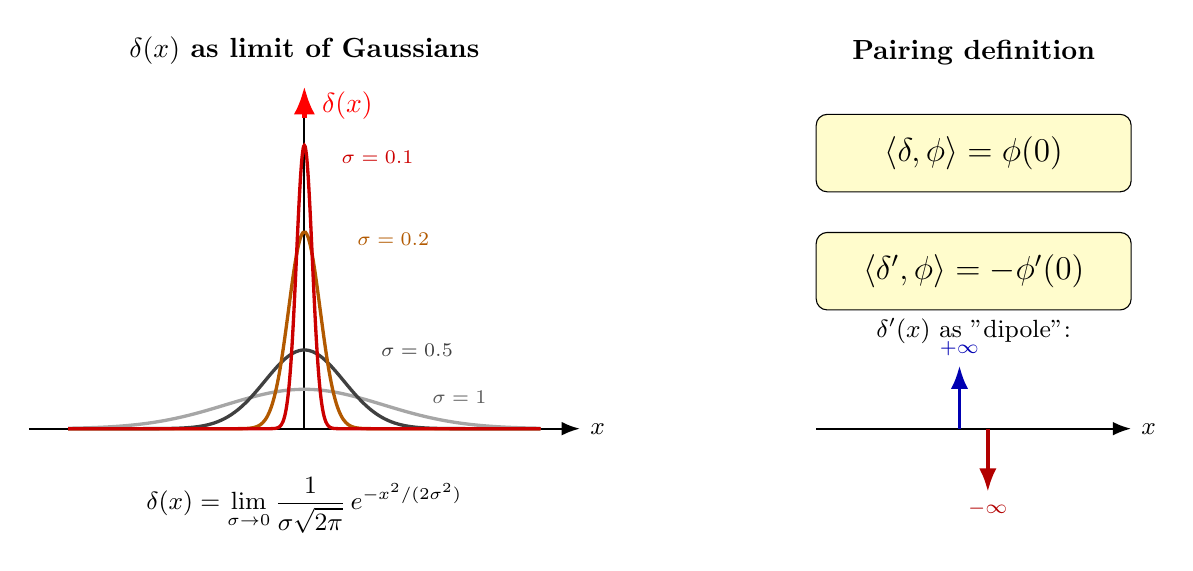
\begin{tikzpicture}[>=Latex]

  % LEFT: delta as limit of Gaussians
  \begin{scope}[xshift=0cm]
    \node[font=\bfseries, anchor=south] at (0, 4.5) {$\delta(x)$ as limit of Gaussians};

    \draw[->, thick] (-3.5, 0) -- (3.5, 0) node[right, font=\small]{$x$};
    \draw[->, thick] (0, 0) -- (0, 4.3);

    % gaussians, with scaled amplitudes to all fit visually
    \draw[gray!70, very thick, smooth, samples=140, domain=-3:3]
      plot(\x, {0.5*exp(-\x*\x/2)});
    \node[font=\scriptsize, gray!70!black, anchor=west] at (1.5, 0.4) {$\sigma=1$};

    \draw[gray!50!black, very thick, smooth, samples=140, domain=-3:3]
      plot(\x, {1.0*exp(-2*\x*\x)});
    \node[font=\scriptsize, gray!50!black, anchor=west] at (0.85, 1.0) {$\sigma=0.5$};

    \draw[orange!70!black, very thick, smooth, samples=200, domain=-3:3]
      plot(\x, {2.5*exp(-12.5*\x*\x)});
    \node[font=\scriptsize, orange!70!black, anchor=west] at (0.55, 2.4) {$\sigma=0.2$};

    \draw[red!80!black, very thick, smooth, samples=300, domain=-3:3]
      plot(\x, {3.6*exp(-50*\x*\x)});
    \node[font=\scriptsize, red!80!black, anchor=west] at (0.35, 3.45) {$\sigma=0.1$};

    % delta limit arrow
    \draw[->, ultra thick, red] (0, 3.95) -- (0, 4.35);
    \node[font=\bfseries, red, anchor=west] at (0.1, 4.1) {$\delta(x)$};

    \node[font=\small, anchor=north, align=center] at (0, -0.5)
      {$\delta(x)=\lim\limits_{\sigma\to 0}\dfrac{1}{\sigma\sqrt{2\pi}}\,e^{-x^2/(2\sigma^2)}$};
  \end{scope}

  % RIGHT: pairing & dipole δ'
  \begin{scope}[xshift=8.5cm]
    \node[font=\bfseries, anchor=south] at (0, 4.5) {Pairing definition};

    \node[draw, fill=yellow!20, rounded corners, font=\large, inner sep=8pt, minimum width=4cm] at (0, 3.5)
      {$\langle\delta,\phi\rangle = \phi(0)$};

    \node[draw, fill=yellow!20, rounded corners, font=\large, inner sep=8pt, minimum width=4cm] at (0, 2.0)
      {$\langle\delta',\phi\rangle = -\phi'(0)$};

    \node[font=\small, anchor=south] at (0, 0.95) {$\delta'(x)$ as "dipole":};
    \draw[->, thick] (-2.0, 0) -- (2.0, 0) node[right, font=\small]{$x$};
    \draw[->, very thick, blue!70!black] (-0.18, 0) -- (-0.18, 0.8);
    \draw[->, very thick, red!70!black] (0.18, 0) -- (0.18, -0.8);
    \node[font=\scriptsize, blue!70!black, anchor=south] at (-0.18, 0.8) {$+\infty$};
    \node[font=\scriptsize, red!70!black, anchor=north] at (0.18, -0.8) {$-\infty$};
  \end{scope}
\end{tikzpicture}
\end{document}
